\documentclass[preprint,times]{aastex61}
\urlstyle{same}
\usepackage{amsmath,amstext}
\usepackage[T1]{fontenc}
\usepackage[figure,figure*]{hypcap}
\usepackage{ragged2e}
\newcolumntype{L}[1]{>{\RaggedRight\hspace{0pt}}p{#1}}
\newcolumntype{C}[1]{>{\centering\hspace{0pt}}p{#1}}

\shorttitle{DC2 Planning Document}
\shortauthors{LSST DESC}

% for \autoref
\renewcommand*\sectionautorefname{Section}
\renewcommand*\subsectionautorefname{Section}
\renewcommand*\subsubsectionautorefname{Section}

\newcommand*{\note}[1]{\textbf{[#1]}}
\newcommand*{\todo}[1]{\note{TODO: #1}}
\newcommand{\infobox}[1]{\begin{center}\fbox{\parbox{0.98\textwidth}{\it #1}}\end{center}}
\newcommand*{\Issue}[2]{\href{https://github.com/LSSTDESC/#1/issues/#2}{#1\##2}}

\begin{document}

\title{DC2 Planning Document}

\author{[Add your name]}
\affiliation{[Add your affiliation]}

\author{R.~Biswas}
\affiliation{Stockholm Oskar Klein Centre, Department of Physics, Stockholm University, SE 106 91 Stockholm, Sweden}

\author{J.~Chiang}
\affiliation{SLAC National Accelerator Laboratory}

\author{S.~Daniel}
\affiliation{University of Washington}

\author{T.~Glanzman}
\affiliation{SLAC National Accelerator Laboratory}

\author{D.~Goldstein}
\affiliation{UC Berkeley}

\author{S.~Habib}
\affiliation{Argonne National Laboratory}

\author{K.~Heitmann}
\affiliation{Argonne National Laboratory}

\author{J.~Peterson}
\affiliation{Purdue University}

\author{E.~Kovacs}
\affiliation{Argonne National Laboratory}

\author{S.~Krughoff}
\affiliation{LSST Project Office}

\author{F.~Lanusse}
\affiliation{Carnegie Mellon University}

\author{P.~Larsen}
\affiliation{Argonne National Laboratory}

\author{R.~Mandelbaum}
\affiliation{Carnegie Mellon University}

\author{Y.-Y.~Mao}
\affiliation{University of Pittsburgh}

\author{P.~Marshall}
\affiliation{SLAC National Accelerator Laboratory}

\author{J.~Sanchez}
\affiliation{UC Irvine}

\author{G.~Sembroski}
\affiliation{Purdue University}

\author{C.W.~Walter}
\affiliation{Duke University}

\collaboration{(The LSST Dark Energy Science Collaboration)}

\begin{abstract}
In this note we describe and document the configurations used for
the second DESC data challenge (DC2) including the validation metrics for
certification of suitability for the science studies described in
the 2017 DESC Science Roadmap document~\citep{SRM:2015}. We provide brief descriptions of the simulation tools used and the outputs that will be provided to the working groups for their DC2 projects. We lay out the schedule for a two-stage production approach and an estimate for the required computing resources.
  
\infobox{\centering This document is in initial draft form. Add your name and expand the text.}
\end{abstract}

\section{Executive Summary for WG Evaluation}

The following document has detailed planning and descriptions for the DC2 simulation configuration. In this executive summary you can find a few tables summarizing the currently chosen configurations.  Please evaluate them to make sure your WG can achieve its analysis goals if these options are used. More detail can sometimes be found in the rest of the document. 

\infobox{This section below should have only summary tables for each relevant set of choices (catalog, image simulation etc) that concisely summarize our choices so that WGs can look at them in \textbf{no more than a few pages} to see if basic choices are consistent with their plans.}

\begin{table}[!htb]
  \centering
  \caption{Extragalactic Catalog Characteristics}
  \label{tab:catalog-options}
  \begin{tabular}{| L{0.2\textwidth}| L{0.75\textwidth}| }
    \hline 
    Property                      & Description/Value   \\
    \hline
    Area & 5000 sq deg \\
    Inpainting method      & Galacticus and Monte Carlo sampling methods\\
    Galaxy information     & Identifier (a unique integer); location (RA, Dec); indicator for central or satellite; scale radius of the disk and bulge components, luminosities.\\  Stellar Mass & Disk, bulge, and total galaxy components.\\
    Redshift information  & Cosmological redshift, observed redshift due to both the Hubble flow and the galaxy's peculiar velocity.\\
    Lensing information  & Shear 1, shear 2; convergence; magnification; lensed position.\\
    Magnitudes                & AB magnitudes of the disk, bulge and total galaxy components in the SDSS $ugriz$ filters, the LSST $ugrizY$ filters and a set of narrow-band top-hat filters designed to provide an approximate SED for each component.  Both absolute magnitudes in the galaxy rest-frame and apparent magnitudes in the observer frame are provided for the SDSS and LSST filters. Magnitudes for the top-hat SED filter set are provided in the rest frame only.  Magnitudes extincted by host galaxy dust and emission-line strengths are computed in post-processing.\\
  Star Formation Rates    & Star formation rate of the disk and bulge components and total galaxy components; Integrated star formation rate; integrated time-Weighted star-formation rate.\\
 Stellar Metallicity          & Mass of metals in stars found in the disk, bulge and total.\\ 
Black-Hole information & Mass of the supermassive black hole; accretion rate of the supermassive black hole. \\
Halo information            & FOF and M$_{200c}$ for host halos\\
Information necessary for IAs (currently being added) & Density fields; halo shapes and angular momentum\\
   \hline
  \end{tabular}
\end{table}

\begin{table}[!htb]
  \centering
  \caption{CatSim Summary}
  \label{tab:catsim-options}
  \begin{tabular}{| L{0.2\textwidth}| L{0.75\textwidth}| }
    \hline 
    Parameter                       & Value   \\
    \hline
    Stars                               & Milky Way model [Bond et al. (2010, ApJ 716, 1), Also see SSim 2017/10/17 meeting]\\
    Transients \& variables  & AGN (damped random walk, independent bands); SNe type Ia; M-dwarf flares; RR-Lyrae; ``Main sequence variability'' (Kepler light curves) \\
    Asteroids                       & None \\
    Dust                               & Milky Way dust model described by SFD model \\
    Proper Motion and Parallax & Removed as not currently handled by DM resulting in astrometric errors. \\
    \hline
  \end{tabular}
\end{table}


\begin{table}[!htb]
  \centering
  \caption{Cadence and Survey options}
  \label{tab:cadence-options}
  \begin{tabular}{| L{0.2\textwidth}| L{0.75\textwidth}| }
   \hline
    Main Survey:       &  \\
    \hline
    Image area         & 300 sq deg \\
    Campaign length    & 10 years \\ 
    Cadence            & \texttt{minion\_1016} WFD proposal visits \\    
    Number of Visits   & $(ugrizy) = (56, 80,184,184,160,160) \times 30$ fields $\sim 27,000$ total \\
    Input              & See Table 1 and 2, plus (stretch goal): natural density of core-collapse SNe, 
                         lensed AGN and lensed SNe\\
    Field Location     & Offset but just including the Extended Chandra Deep Field South Deep Drilling Field \\
    Dithering          & Realistic large dithers and rotations  \\
    \hline
    Ultra-DDF:         &  \\
    \hline
    Image area         & $\sim1.25$ sq deg (3 rafts, 27 sensors, 4600 sq arcmin, 
                         15\% of a full FoV), embedded in one corner of the main 
                         survey region \\
    Campaign length    & 10 years \\ 
    Cadence            & \texttt{minion\_1016} 
                         DDF proposal visits (re-arranged from year to year to emulate enhanced cadences),
                         including visits labeled WFD from the \texttt{minion\_1016} WFD proposal \\
    Number of Visits   & $\sim 20,000$ total \\
    Input              & See Table 1 and 2, plus: over-abundance of lensed 
                         AGN ($\gtrsim 1000$, 0.2/sq arcmin) and lensed 
                         SNe ($\gtrsim 1000$, 0.2/sq arcmin), and: 
                         $\sim6\times$ over-abundance of SNe Ia (25000, 5/sq arcmin), 
                         core-collapse SNe (similar) \\
    Field Location     & Extended Chandra Deep Field South Deep Drilling Field \\
    Dithering          & WFD visits dithered and rotated (since these are also main survey visits). 
                         DDF visits to have small (chip-scale) dithers, and realistic rotations (same as for WFD).   \\
    \hline
  \end{tabular}
\end{table}

\begin{table}[!htb]
  \centering
  \caption{DC2 image features}
  \label{tab:image-options}
  \begin{tabular}{| L{0.2\textwidth}| L{0.75\textwidth}| }
    \hline 
    Parameter                                      & Value   \\
    \hline
    Bands                                           & $ugrizy$   \\
    Galaxy morphology                      & Compound Sersic Galaxies from inpainting model; imSim version also includes random walk knot model for irregular morphology \\
    Lensing & Lensing and magnification applied to galaxies \\
    Sky model & PhoSim: PhoSim sky model; ImSim: ESO sky model; both include moonlight\\
    Weather & PhoSim: skyglow and clouds; ImSim: none \\
    Atmosphere                           & Ray-traced atmosphere; includes differential chromatic refraction \\
    Optics                                     & PhoSim: Full raytracing through LSST optics; ImSim: Aberrated optical phase screen \\
    Sensor                   &  Brighter-Fatter, Tree-rings (for imSim mixed focal plane), cosmic rays, bleeding, and x-talk.  Hot columns and defects handled by masking. \\
    Readout                                  & Output includes pre-readout image (e-image) and full readout physics (amplifier image)\\
     \hline
  \end{tabular}
\end{table}

\begin{table}[!htb]
  \centering
  \caption{Final Output Format}
  \label{tab:output-options}
  \begin{tabular}{| L{0.2\textwidth}| L{0.75\textwidth}| }
    \hline 
    Parameter                    & Value   \\
        \hline
    Output format             & DM output products,Tables in qserve prototype (at least for transients) and Dask/Pandas based dataframes \\
    Output products         & All DM output including shape measurement on coadds in databases/dataframes, Truth tables for stars and galaxies, final matched catalog with truth information. \\
    Non-Default columns & Several photometry magnitudes and fluxes with associated errors in micro-Janskys. \\
    Matched truth metadata & Important items will include: Extincted and non-extincted true magnitudes, Halo mass, peculiar and Hubble velocity \\
   \hline
  \end{tabular}
\end{table}


\begin{table}[!htb]
  \centering
  \caption{Rough User timeline}
  \label{tab:User-Timeline}
  \begin{tabular}{| L{0.2\textwidth}| L{0.75\textwidth}| }
    \hline 
    Parameter                    & Value   \\
    R1.1 Production Start                & Mid/End January \\
    R1.1 Data Release and Introduction   & Beg/Mid February (SLAC Collaboration Meeting) \\
    R1.1 Validation period               & Presentations after one month of work by WGs in mid March \\
    R2.0 Production starts                & End of March \\
    R2.0 Data release                    & Mid/End of June \\
    R2.0 Early Analysis                  & Mid July (Collaboration Meeting) \\
   \hline
  \end{tabular}
\end{table}


\clearpage

\section{Introduction}

At the June 2017 Stony Brook collaboration meeting the SSim group
surveyed and discussed with the analysis working groups (WG) their
needs for DC2 production.  The WGs were presented with a baseline DC2
configuration and then they presented their plans for DC2 analysis
along with requests for additional features or configuration options
which were currently not present. A very brief summary of the working group plans is given in \autoref{sec:plans}.

This document summarizes the consensus list of the needed parameters
and configuration options and serves as a record of the options used
in the DC2 production.  Additionally, in this document we specify a set of validation 
tests that are used to ensure that the produced catalogs satisfy the requirements of the working groups. The validation tests will be first carried out on down-scaled versions of the DC2 catalogs for all production stages (extra-galactic, image, and DM catalogs).
The document also presents our strategy of staging the DC2
production along with which tools will be used for each part and a timeline.
 
\section{Planned uses for the DC2 Simulation}
\label{sec:plans}

Brief summaries of how the analysis and technical working groups plan to use the DC2 simulations are below.  For each planned project, the brackets indicate whether the project will use the smaller-area image simulations [I], the larger-area extragalactic catalog [C], or both [C,I].  In this case, `C' means that the groups will use the extragalactic catalog directly (and/or with custom modifications introduced by them,), but do not expect the CS working group to do any further emulation of what those extragalactic catalogs would look like after producing image simulations.
\begin{itemize}
\item Galaxy clusters (CL):
\begin{enumerate}
%\item[{[I]}] Studying how observational systematics affect the performance of cluster-finding algorithms (as quantified by studying the purity/completeness, centering, mass-observable scatter, etc.), by comparing the results of cluster-finding on the processed catalogs derived from the simulated images with the true halo catalogs.
\item[{[I]}] Studying how observational systematics affect the performance of cluster-finding algorithms.
\item[{[I]}] Testing the impact of blending and shear estimation biases on cluster mass reconstruction.
\item[{[C,I]}] Analyzing the images and snapshot data to understand the impact of observational systematics on cluster lensing profiles. 
\end{enumerate}
\item Large-scale structure (LSS):
\begin{enumerate}
\item[{[C]}] Investigating methods for optimally-selecting galaxies for large-scale structure analysis using photometric redshift posteriors, and the impact on cosmology constraints.
\item [{[C]}] Similar to the above, but considering selection based on colors/magnitudes, such as extreme emission line galaxy selection.
\item [{[C,I]}] Testing LSS analysis pipeline (including angular power spectrum estimation with mode projection for systematics) for selected galaxy subsamples.
\item[{[I]}] Measuring magnification bias in the presence of realistic systematics.
\item[{[I]}] Testing the impact of a selected set of theoretical and observational systematics on two-point clustering measurements.
\end{enumerate}
\item Photometric redshifts (PZ):
\begin{enumerate}
\item[{[C]}] Testing the impact of incompleteness in spectroscopic training samples on the quality of photometric redshift estimates, and the impact on various DESC science cases.
\item[{[C]}] Testing methods for inferring ensemble redshift distributions for photo-$z$-selected samples using cross-correlation analysis, including magnification and realistic nonlinear galaxy bias models.
\end{enumerate}
\item Strong lensing (SL):
\begin{enumerate}
\item[{[I]}] Extending an existing machine learning framework originally developed for galaxy-galaxy strong lenses to detect strongly lensed quasars, and test its effectiveness on image simulations.
\item[{[I]}] Investigating the prospect of measuring time delays using the shock breakout light curves of  high-redshift, strongly lensed core collapse supernovae from LSST.
\item[{[I]}] Evaluating supervised and unsupervised methods for double source-plane lens finding in wide-field optical imaging surveys, and forecasting their cosmological constraining power in LSST.
\item[{[C]}] Investigating the effect of the rolling cadence on the lensed supernova science case.
\item[{[I]}]  Full end-to-end cosmology forecast using strongly lensed supernovae from the ultraDDF.
\end{enumerate}
\item Supernovae (SN):
\begin{enumerate}
\item[{[C]}] Optimizing the WFD observing strategy for recovery of Type Ia supernova light curves and ease of SN classification.
\item[{[I]}] Testing transient classification methods, including the impact of artifacts in the image processing.
\item[{[I]}] Testing the recovery of strongly-lensed supernovae and AGN (joint project with SL working group) and the ability to measure light curves in the presence of a foreground object, given realistic blending.
\end{enumerate}
\item Weak lensing (WL):
\begin{enumerate}
\item[{[I]}] Validating weak lensing shear two-point correlation measurements in the presence of realistic image-level systematics and survey masks.
\item[{[C,I]}] Testing the full end-to-end weak lensing cosmology inference pipeline, from images to cosmological parameters, including marginalization over both observational and theoretical systematics.
\item[{[I]}] Investigating the impact of realistic levels of blending on weak lensing galaxy samples selection and shear biases.
\item[{[I]}] Testing the effectiveness of PSF modeling routines, and the impact of residual systematics on weak lensing.
\item[{[C]}] Testing the hierarchical Bayesian mass reconstruction from tomographic weak lensing and galaxy clustering in LSST.
\item[{[C]}] Evaluating the impact of the ability to model over small-scale theoretical uncertainties (nonlinear bias, assembly bias, etc.) in the 3x2pt analysis, and push to smaller scales in the analysis.
\end{enumerate}
\item Sensor Anomalies (SA):
\begin{enumerate}
\item[{[C,I]}] Validate the simulation and the  correction of the Brighter-Fatter (BF)  effect .
\item[{[I]}]  Evaluate the acceptable level of  BF residual in key analysis . 
\end{enumerate}
\end{itemize}

\section{DC2 Simulation Pipeline and Workflow}

\begin{figure}[!htb]
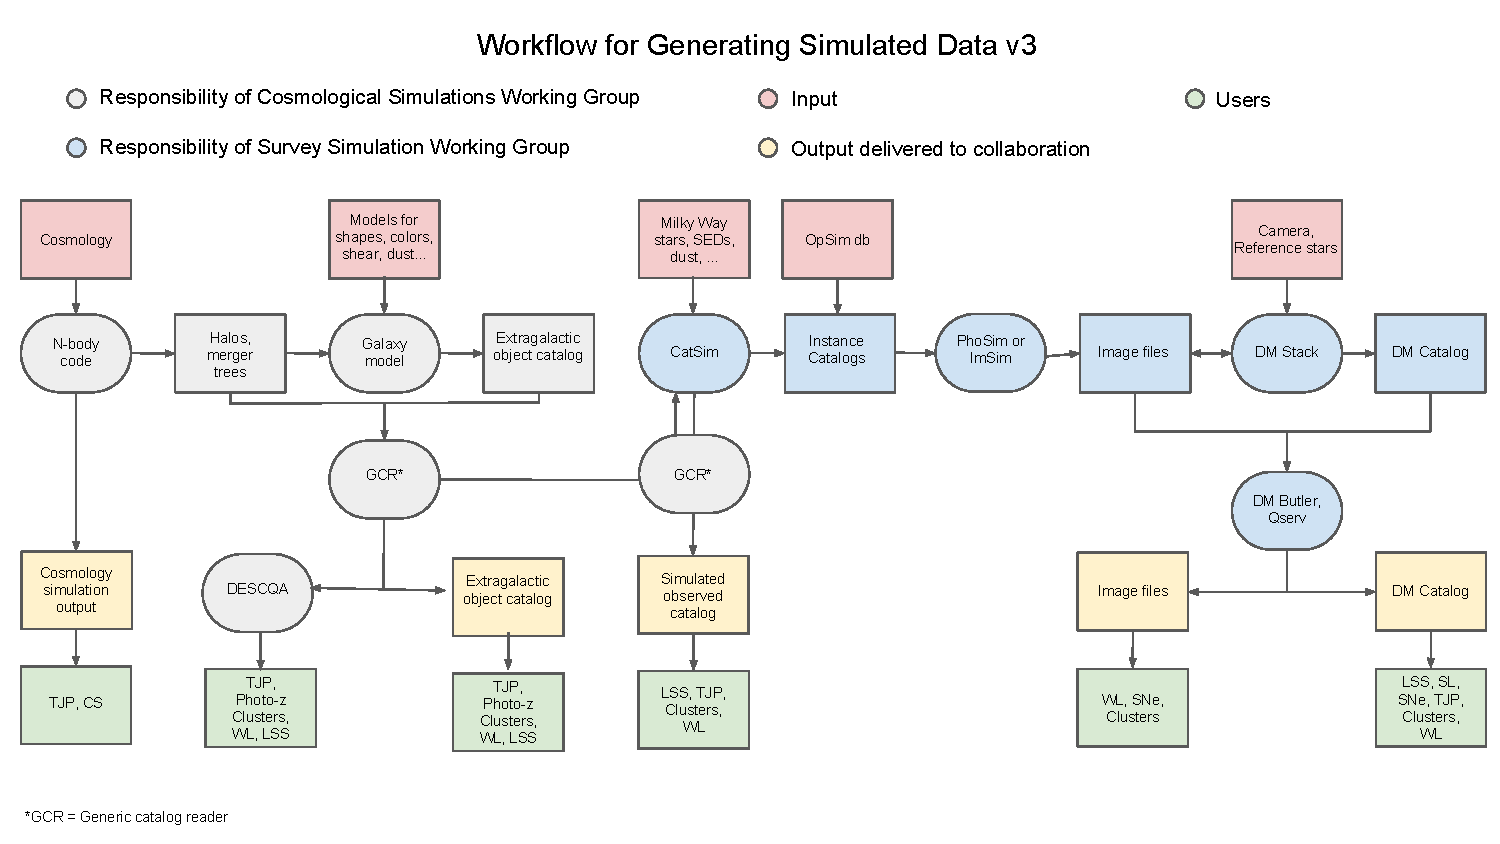
\includegraphics[width=1\textwidth]{Catalog_Simulation_Workflow}
\caption{\label{fig:workflow}Workflow diagram showing the full end-to-end process for generating the simulated DC2 catalogs. Colors show inputs in red, outputs in yellow, users in green, and working groups responsible for the workflow pieces in gray (CS) and blue (SSim).}
\end{figure}

The generation of the simulated catalogs -- extragalactic, CatSim, and DM catalogs -- involves many steps that need to be implemented and tested. \autoref{fig:workflow} shows an overview of the end-to-end generation of the simulated DM catalogs, starting with the N-body input simulations. The challenges for generating the diverse simulated catalogs include but are not limited to:
\begin{itemize}
\item Development, scaling, and testing of all necessary simulation tools; in particular, methods for generating the extragalactic catalogs (currently Galacticus, variants thereof, and empirical techniques) and methods for generating the image simulations (currently PhoSim and ImSim); these are tasks that have to be carried out by the CS, CI, and SSim groups (see Sections~\ref{sec:mocks} and \ref{sec:imagesims})
\item Developing workflows to enable straightforward generation of the extragalactic and simulated observed catalogs and the following image generation with PhoSim or ImSim; this is a task that needs to be carried out by CS, CI, and SSim (see \autoref{sec:worklfow})
\item Processing of the resulting catalogs through the DM stack to generate the DM catalogs, this task is carried out by CI and SSim
\item Enabling easy access for the analysis working groups to the different data products that are generated, this task is currently carried out by CS, CI, and SSim (see \autoref{sec:output})
\item Validation of the outputs generated at the different stages; here, very active collaboration with the analysis working groups is essential (see \autoref{sec:validation})
\end{itemize}

\autoref{fig:workflow} shows on the left hand side the generation of the extragalactic and simulated observed catalogs that will be accessed via the Generic Catalog Reader (GCR) which has been developed by the CS group. A more detailed discussion of the GCR is provided in \autoref{sec:gcr}. On the right hand side, the generation of instance catalogs, image files, and the final DM catalogs is shown. For the generation of DC1, the collaboration relied on extragalactic catalogs from the Millennium simulation which were already embedded in the CatSim framework. Therefore, during the DC1 simulation production SSim and CI were only concerned about the right hand side of the workflow, starting with CatSim. In the meantime, CS developed the left hand side of the workflow, including an automated validation framework, DESCQA~\cite{descqa} and the GCR. For DC2 the two parts of the workflow have to be now connected since the Millennium extragalactic catalog is limited in size and does not provide shear measurements. 

As we will describe in more detail in \autoref{sec:timeline} we will first develop the full end-to-end pipeline for a downscaled version of the DC2 extragalactic catalog (called protoDC2) to provide ample opportunities for testing and validation of all steps in the pipeline and the resulting catalogs.

\subsection{Production Strategies: Workflow Approaches for the Catalog Generation}
\label{sec:worklfow}
For image simulation production at NERSC, the plan is to use the Pegasus workflow system to orchestrate the execution of the PhoSim or imSim jobs.  This will involve working with NERSC computing support in order to have a central installation of the HTCondor batch system that Pegasus uses to manage pipeline execution.  Since substantial development may be required to get Pegasus/HTCondor to run efficiently at NERSC, we will have the SLAC workflow engine, which was used for the DC1 image data generation, available as a backup. 

Because a single ImSim or PhoSim job is too small to fill an entire Cori-KNL node, ``glide-in" technology will be employed to make efficient use of the computing resources.  In essence, a glide-in is a batch job that runs under the native batch system, e.g., SLURM in the case of NERSC.  The glide-in executes a particular configuration of the HTCondor client code, making the node or nodes appear as an HTCondor compute pool.  Pegasus jobs are then dispatched to one or more glide-in jobs via the normal HTCondor queuing scheme.  Note that a single glide-in instance may control one or more KNL nodes and can run multiple Pegasus jobs simultaneously.

\section{DC2 Extragalactic Catalog}

\subsection{CosmoDC2: Cosmological Simulation Set-up and Content}
\label{cosmoDC2}

The N-body simulation underlying the DC2 extragalactic catalog, is the so-called Outer Rim simulation, carried
out with the Hardware/Hybrid Cosmology Code (HACC) on the ALCF supercomputer Mira. The Outer Rim simulation evolves more than 1 trillion particles in a $(4225$Mpc$)^3$ volume, leading to a mass resolution of $m_p=2.6\cdot 10^9$M$_\odot$. The cosmology underlying the Outer Rim simulation is close to the best-fit WMAP-7 cosmology, given by the following parameters: $\omega_{\rm cdm}=0.1109$, $\omega_{\rm b}=0.02258$,
$n_s=0.963$, $h=0.71$, $\sigma_8=0.8$, $w=-1.0$. We have stored 99 snapshots between $z=10$ and $z=0$ evenly spaced in $\log (a)$. The resulting data file is more than 4PB large and is kept on HPSS at the ALCF. Due to its size, this dataset cannot be made available to DESC. Additional data products include at the same 100 redshifts:
\begin{itemize}
\item Downsampled raw particle files storing 1\% of the full particle dataset; this dataset can be used to generate density fields for intrinsic alignment modeling. 
\item Matter power spectra
\item {\it FOF halo catalogs with a linking length of $b=0.168$ down to 20 particles per halo}
\item SO catalogs (M$_{200c}$) for FOF halos with at least 1000 particles
\item Halo core catalogs (once a halo has formed and reached a size of 100 particles, we identify 10 particles closest to its center and follow them for the rest of the simulation, even if they do not belong to a halo)
\item Particle and halo ids for all particles in halos
\item Particles in halos with more than 100,000 particles
\item 1\% of particles in halos (at least 5 particles per halo)
\item Merger trees built from the FOF halo catalogs and cores
\end{itemize}
Additional halo properties that have been requested to enable intrinsic alignment modeling are:
\begin{itemize}
\item Shape eigenvectors
\item Angular momenta
\end{itemize}
For the snapshots between $z=1.5$ and $z=0$ we also identified subhalos for the cluster sized halos (more than 100,000 particles). This was done in part to show that the core tracking solution for specifying galaxy positions in halos is actually more accurate. Some details on this approach can be found in the protoDC2 DESC Note~\citep{protoDC2} and in \cite{korytov}. Currently, only the FOF halo information is included in the protoDC2 dataset (we marked this entry in italics). Additionally, the SO information, the shape eigenvectors, and the angular momenta have been requested. These quantities are evaluated with the latest version of our halo finder. Density field information has also been requested and can be generated from the down-sampled particle snapshots. Outside of the simulated DC2 catalog work, other requests have been made (e.g. for access to the merger trees) but this discussion is beyond the scope of this document. A major bottleneck for making more data products available is shortage of storage. All the data is currently stored at Argonne. Generating additional halo information beyond the list given above is costly due to the large datasize so would have to be considered very carefully. 

\subsection{CosmoDC2: Extragalactic Catalog Generation}
\label{sec:mocks}
Based on the merger trees extracted from the N-body simulation, the next step is to populate the simulation with galaxies. A range of methods can be used for this task, several of them are described in the Appendix of \cite{descqa}. For the main DC2 production run we will use a combination of methods based on a semi-analytic approach as implemented in Galacticus and a Monte Carlo sampling approach which we briefly describe in the following.
A more detailed description of our approach is given in \cite{protoDC2} which focuses on the generation of the protoDC2 extragalactic catalog.

\subsubsection{Galacticus}

Galacticus is a semi-analytic model of galaxy formation developed by Benson~\cite{benson}. It is used here to populate the simulation halos with galaxies in post-processing. Galacticus takes as input merger trees and, along each branch of each tree, solves a set of differential equations which describe the evolution of coarse-grained properties of the galaxy that forms within that branch. These properties include both physical quantities such as the masses of stars and gas in the galaxy, and directly observable quantities such as luminosities. This differential evolution is supplemented with impulsive events to describe galaxy mergers. The physics modeled by Galacticus includes the cooling of gas in the circum-galactic medium and its inflow into galaxies, star formation, supermassive black hole growth, feedback processes powered by both supernovae and active galactic nuclei, metal production, and galaxy merging. 

\subsubsection{Monte Carlo Sampling Approach}
Semi-analytic models such as Galacticus provide realistic levels of complexity in the galaxy--halo connection that are needed to meaningfully test the analysis pipelines cosmological surveys. This complexity comes at significant expense: a complete run of Galacticus for protoDC2 took $\sim 420$ core hours to complete ($\sim$ 250k NERSC hours on the KNL partition of Cori and 250k hours on the local Argonne cluster Phoenix, for the NERSC hour definition see \autoref{compute} on computing allocation needs.) As DESC working groups have diverse needs that require generation of many different versions of mock catalogs, this creates a computational challenge that is sharpened further by the common demands for simulations of very large volume.

Fortunately, Monte Carlo resampling techniques can be used to "scale up" synthetic catalogs to much larger simulations than those used for the original catalog production. We have designed a publicly available python package {\tt Galsampler} for this purpose. The technique begins with a baseline synthetic sky produced in a modest-volume simulation. For every distinct halo in some final target simulation, {\tt Galsampler} identifies a halo of similar properties in the original simulation, and transfers the entire resident galaxy population from the source to the target halo, preserving the host-centric positions and velocities of each galaxy. This method allows us to populate a new, larger volume simulation with a new galaxy catalog that largely preserves the complexity of the original catalog, without having to rerun the semi-analytic model. This approach also enables us to use different approaches for modeling galaxies on top of the N-body simulation in an easy and fast way and therefore deliver catalogs based on different methods easily. These methods can even include hydrodynamical approaches that are too expensive to run on large cosmological volumes. {\tt Galsampler} therefore will enable the working groups to use different inpainting methods to test that the biasing/non-linear modeling approaches are sufficiently general and to which scales they work. 

\subsubsection{Lightcone Production and Shear Measurements}

For the lightcone generation and shear measurement approach we follow closely the description provided in \cite{protoDC2}. The main difference will be that with the larger sky area covered (the current aim is 5k sq degrees) the flat sky approximation employed for protoDC2 will not hold any longer. We are currently implementing and testing 

\subsection{CosmoDC2: Extragalactic Catalog Content}

In the following we provide a compact list of the content of the extragalactic catalog. The current plan is that the extragalactic catalog will cover 5k sq degrees. Some of the details are still being refined during the validation phase of the protoDC2 catalog and the most comprehensive and up-to-date version of this list can be found in a Google  spreadsheet\footnote{\url{https://docs.google.com/document/d/1rUsImkBkjjw82Xa_-3a8VMV6K9aYJ8mXioaRhz0JoqI/edit}}. This spreadsheet is being continuously updated by the CS Working Group. 


\begin{itemize}
\item Galaxy information: identifier (a unique integer); location (RA, Dec); indicator for central or satellite; scale radius of the disk and bulge components, luminosities.
\item    Stellar Mass of the disk, bulge, and total galaxy components.
\item Redshift information: Cosmological redshift, observed redshift due to both the Hubble flow and the galaxy's peculiar velocity.
\item Lensing information: Shear 1, shear 2; convergence; magnification; lensed position.
\item    Magnitudes: AB magnitudes of the disk, bulge and total galaxy components in the SDSS $ugriz$ filters, the LSST $ugrizY$ filters and a set of narrow-band top-hat filters designed to provide an approximate SED for each component.  Both absolute magnitudes in the galaxy rest-frame and apparent magnitudes in the observer frame are provided for the SDSS and LSST filters. Magnitudes for the SED filter set are provided in the rest frame only.
Dust-corrected magnitudes and emission-line strengths are computed in post-processing.
\item    Star Formation Rates: Star formation rate of the disk and bulge components and total galaxy components; 
Integrated star formation rate; integrated time-Weighted star-formation rate.
\item  Stellar Metallicity: Mass of metals in stars found in the disk, bulge and total. 
\item    Black-Hole information: Mass of the supermassive black holel; accretion rate of the supermassive black hole. 
\end{itemize}
 
For the CosmoDC2 catalog all the information will be delivered via lightcone outputs. In addition to enable some specific tests regarding intrinsic alignment modeling we will provide two snaphots at $z\sim 0.06$ and $z\sim 0.9$ for protoDC2.

\subsection{Remaining Tasks}

This is a brief summary of tasks that have been identified so far during the protoDC2 validation phase that need to be still carried out before the DC2 production can start. Most of these tasks are integration of already developed measurements into the catalogs or improved scaling of the catalog generation tools. Validation tests are not listed here but rather discussed in a separate section below.

\begin{itemize}
\item Integration of halo properties (M$_{200c}$, shape measurements, angular momentum) into released catalog
\item Weak lensing cluster maps
\item Finalize large angle treatment for weak lensing shear measurements
\item Density field generation
\item Data organization within the catalog that allows scalable ingestion into CatSim. This will be achieved via Healpix or appropriate HDF5 data organization. 
\end{itemize}

\section{DC2 CatSim Catalog}

After the extragalactic catalogs have been generated, instance catalogs are needed to serve as input to the image simulation tools. Currently, the CatSim framework is used to carry out this step. CatSim enables access to a range of LSST specific data, including: Position on LSST focal plane (mm), Pixel position on LSST focal plane, Geocentric apparent position,            
Luminosity distance, E(B-V) from Milky Way dust, $A_V$ from Milky Way dust, LSST/SDSS magnitudes/fluxes+uncertainty. Some of these are specified by the user before the catalog is processed through CatSim and might be targeting a very specific science goal. \autoref{tab:catsim} provides a summary of the inputs to CatSim and the resulting outputs.

\begin{table}[!htb]
  \centering
   \caption{CatSim catalog content}
  \label{tab:catsim}
  \begin{tabular}{| l| l| }
    \hline 
Inputs        &               CatSim outputs \\
\hline
RA, Dec, observation metadata    &   Position on LSST focal plane (mm)\\
RA, Dec, observation metadata  &  Pixel position on LSST focal plane \\
RA, Dec, observation metadata         &  Geocentric apparent position  \\
Redshift, cosmology                  &    Luminosity distance\\
RA, Dec         &   E(B-V) from Milky Way dust   \\
RA, Dec                &   Av from Milky Way dust\\
SED, SED normalization                &   LSST magnitudes/fluxes\\
SED, SED normalization, observation metadata       & LSST magnitude/flux uncertainty  \\
SED, SED normalization, observation metadata              &   SDSS magnitudes/fluxes  \\
SED, SED normalization, observation metadata      &   SDSS magnitude/flux uncertainty \\
   \hline
  \end{tabular}
\end{table}

\subsection{Remaining Tasks}
For the CatSim catalogs the main challenge is to enable a fast data ingestion for the extragalactic catalogs. Timing tests will be carried out during the protoDC2 validation phase.

There are various other tasks that will be needed for full DC2 production, as well as several that should be implemented before Run~1.1 data generation:
\begin{itemize}
\item The {\tt generateDc2InstCat.py} script needs to be updated to produce "imsim-style" instance catalogs.  These differ from the phosim versions in that the object entries are given with ICRS coordinates.
\item Time-varying AGN need to be implemented using protoDC2 catalog inputs.
\item Extraction of Truth Tables from CatSim.  The contents of these tables needs to be specified, e.g., top-of-the-atmosphere {\em ugrizy} magnitudes, galaxy shape and WL distortion parameters, etc..  For time-varying objects, we will need entries for every visit in which they appear, whereas non-varying objects would just need a single entry for the full survey.
\item A specific region of the sky for the 300 sq degrees of DC2 that encompasses a DDF for the time-domain studies.
\item Dithering implementation to apply to the baseline opsim cadence. This likely entails a different dithering strategy for the DDF-specific visits vs the strategy applied to the other visits.
\end{itemize}

\section{DC2 Image Files and DM Catalog}

\subsection{DC2 Image Simulation Tools}
\label{sec:imagesims}
\subsubsection{PhoSim}
PhoSim is a first-principles physics simulator designed to produce realistic astronomical images using a detailed Monte Carlo approach.  This includes representing the relevant physics of light and electron propagation through the atmosphere, optics, sensors, and readout system.  PhoSim compiles a detailed representation of the site \& instrument characteristics of LSST (and other observatories) that is included in the calculation.  PhoSim has been validated through thousands of validation tests that compare observable signatures with real data or analytic predictions.  PhoSim is the natural tool to use when making simulations that include all the complexity of real data.  It is also useful as a tool to probe the relevance of individual physical effects on a specific cosmological measurements by using the configurable modular options that turn on or off individual effects.   


\subsubsection{ImSim}

ImSim provides LSST simulation capabilities using the open-source GalSim software package and utilities from LSST DM.  GalSim was designed quite differently from PhoSim.  Rather than being designed for end-to-end full physics-based simulations, it is designed to be a modular simulation toolkit that allows easy swapping of modules with different descriptions for galaxies, PSFs, detector effects, etc.  Some of the options for e.g. PSFs and detector effects are simple approximations while others correspond to full physics (e.g., the silicon models recently added by Craig Lage, or ray-tracing stochastic atmospheres by Josh Meyers).  Doing ``kitchen sink''-style simulations with ImSim in its current state would require omitting some physical processes that happen naturally in PhoSim.  However, it is quite naturally suited for investigations of what happens when turning specific effects on or off.  The speed depends sensitively on the chosen fidelity for certain aspects of the simulation processes (e.g., fully realistic galaxy morphology vs.\ parametric models; ray-tracing through stochastic atmospheres vs.\ using parametric PSF models; simple pixel response vs.\ the full silicon model for LSST).


\subsection{DC2 Catalog and Image Configuration Options}

The options chosen for the DC2 production are for the most part a
further specification or refinement on the specifications of the challenge datasets
table in the SRM. 

\autoref{tab:image-options} describes the choice of options for
production as decided after consultation and discussion among the
working groups and those coordination the DC2 production.

\begin{table}[!htb]
  \centering
   \caption{Catalog and image production options}
  \label{tab:image-options-2}
  \begin{tabular}{| l| l| }
    \hline 
    Parameter                       & Value   \\
    \hline
    Catalog and Image area  & 300 sq deg \\
    Bands                             & ugrizy   \\
    Number of Visits per band  &  (ugrizy) = (56, 80,184,184,160,160) \\
    Cadence                         & OpSim WFD with embedded DDF and twinkles fields\\
    Input                              & Outer rim catalog +MW stars model \\
    Sky Model                      & Basic OpSim Model \\
    Dithering                       & Random translational and rotational  \\
    Sensor Effects                & Basic sensor effects (saturation, tree-rings, brighter-fatter) \\
    Readout type                 & E-image and amplifier readout available \\
    \hline
  \end{tabular}
\end{table}

The command files which implement this configuration can be found in
\autoref{sec:command-file}.  The CatSim query commands can be
found in XXX \todo{Can we document this?}.

\subsection{DC2 Catalog Content}
\begin{itemize}
\item Visit metadata: pointing information, seeing, sky bg, noise, etc. from calexps and the opsim db.
\item deepCoadd-results: object catalogs from measuring coadds, including photometry, various shape measurements, and analysis flags (a few hundred columns per object, DC1 had about 11M objects)
\item forced: forced photometry flux catalogs at coadd object locations 
\end{itemize}



\section{Timeline}
\label{sec:timeline}

\begin{figure}[t]
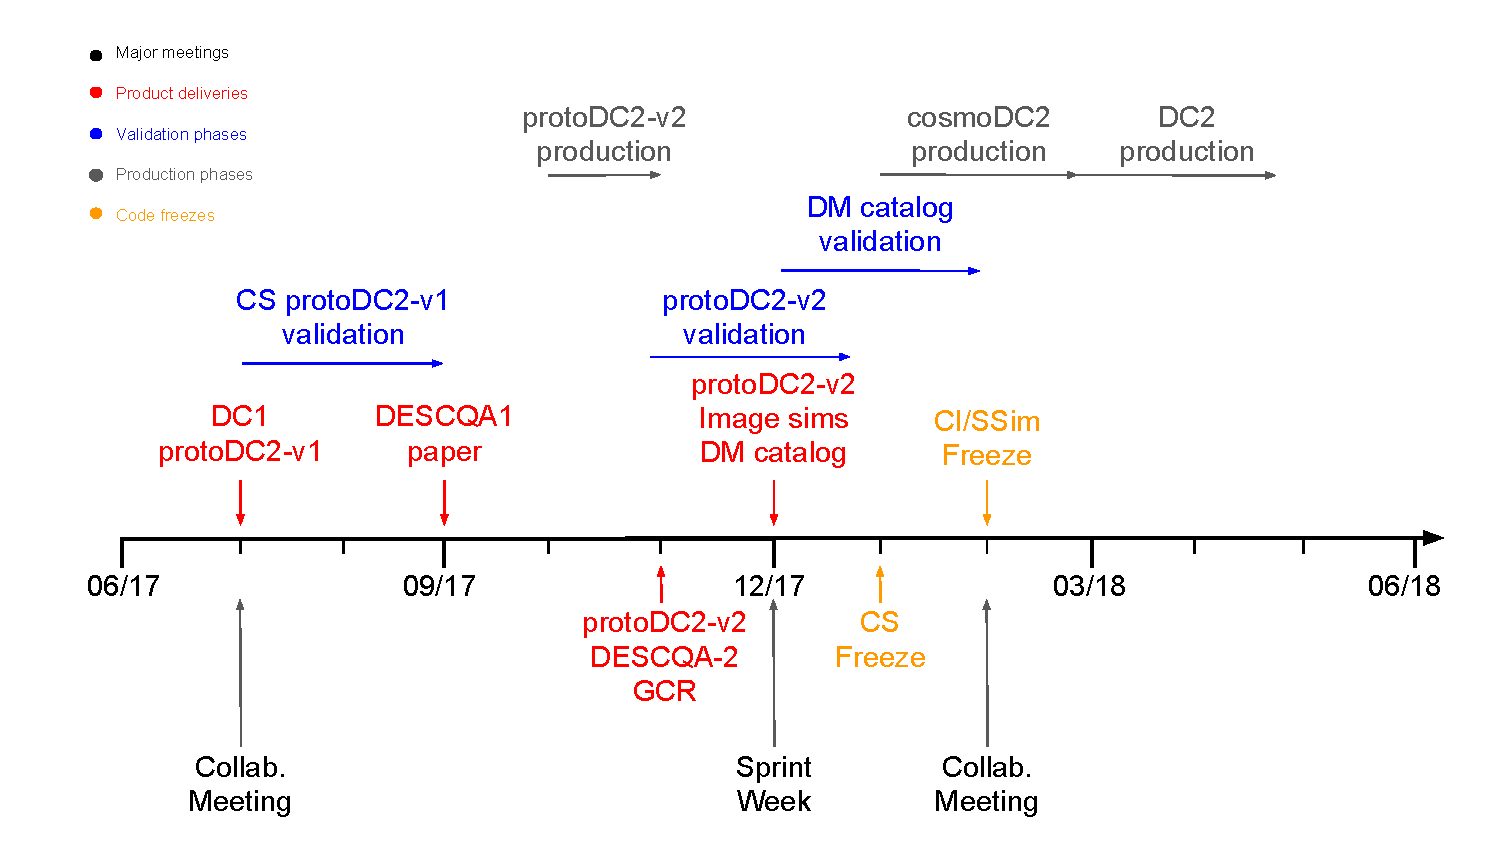
\includegraphics[width=1\textwidth]{DC2timeline}
\caption{\label{fig:schedule}Schedule for delivering the two stages of the DC2 production. A first, downsized set
of catalogs will be delivered by December 2017 to enable the validation of the catalogs by the analysis working groups. This validation process should be concluded by the Spring Collaboration Meeting in February 2018 at which point full DC2 production would start.}
\end{figure}

In order to enable the generation of fully validated and tested catalogs for DC2 at all stages (extragalactic to DM catalogs) it is important to develop a staged production approach that starts with a smaller dataset for proto-typing the workflow and production set up. An efficient production schedule has to interleave the generation of the different catalogs with extensive validation tests. \autoref{fig:schedule} outlines a possible schedule for the creation of the full DC2 catalog suite, including extragalactic catalogs, image simulations, and DM catalogs. The schedule is built around the delivery of products at the major DESC Collaboration Meetings and the Sprint Week in the fall of 2017. We show products that will be delivered to the collaboration at certain dates in red, validation phases during which the collaboration can verify that the catalogs have all desired features and agree at the required level of accuracy with observational data in blue, and actual production phases in gray. We also mark the dates where the production tools for the different catalogs will be frozen and no new features will be added.

The schedule shown in the figure focuses on the DC2 development and has to start necessarily with the production and delivery of the extragalactic catalog. During this first stage, the collaboration will work with the already available DC1 catalogs to not only generate science results but also to learn how to access and interact with the DM catalogs. The DC1 data set 
has been delivered to the collaboration in Stony Brook and DC1 analysis tasks will be carried out during the Fall Sprint Meeting.

In the following, we provide very brief descriptions of the different stages and deliverables to arrive at the full DC2 catalog in May 2018. These milestones are also listed in \autoref{tab:milestones}.

\begin{table}[!htb]
  \centering
  \caption{Initial set of DC2 Milestones. A ``milestone'' is either a product with a delivery date (i.e.\ an SRM ``deliverable''), or an event with a date of occurrence (e.g.\ a review, or a date release). Major milestones are marked in bold.}
  \label{tab:milestones}
   \fontsize{9pt}{10.5pt}\selectfont 
  \begin{tabular}{|L{0.3\linewidth}|C{0.11\linewidth}|L{0.53\linewidth}|}
    \hline 
    Milestone (Product or Event)             & Delivery Date & Notes \\
    \hline\hline
    protoDC2-v2 Extragalactic Catalog        & 10/31/2017 & DESC Note describing the catalog and its generation\\
    DESCQA2 \& \textsc{GCRCatalogs}          & 10/31/2017 & \\
    Run 1.0 (protoDC2-v2) Instance Catalogs  & 12/08/2017 & \\ 
    Run 1.0 Truth Tables                     & 12/08/2017 & To enable verification of Run 1.0 DM measurements. \\
    Run 1.0p (PhoSim) Images                 & 12/08/2017 & \\
    Run 1.0p DM Catalogs                     & 12/08/2017 & Aiming to have Run 1.0 products at the Argonne Sprint Week. \\
    Run 1.1 (protoDC2-v3) Instance Catalogs  & 01/12/2018 & Includes the required 1) cadence and dithering, 2) time domain objects. \\
    SSim Image Simulation Pipeline           & 01/12/2018 & Including algorithms, configurations. ``SSim Code Freeze,'' (no new ImSim or PhoSim features), start Run 1.1 image simulation. \\
    Run 1.1p/i (PhoSim \& ImSim) Images         & 01/19/2018 & 1 week to produce Run 1.1p and Run 1.1i images, from identical instance catalogs. \\
    CI DM DRP Pipeline                       & 01/19/2018 & Including algorithms, configurations. ``CI Code Freeze'' (no new DM features), start Run 1.1 DM processing. \\
    Run 1.1 Truth Tables                     & 01/26/2018 & In time to enable verification of Run 1.1 DM measurements. \\    
    Run 1.1p/i DM Catalogs                      & 01/26/2018 & 1 week to process the Run 1.1 images, to enable first validation test results (on DM catalogs) by the start of the winter collaboration meeting. \\ 
    DM Catalog Validation Test Suite         & 02/02/2018 & Developed against DC1 and Run 1.0 DM catalogs, and completed in time to be run on the Run 1.1 DM catalogs, starting at the SLAC meeting. \\ 
    CS Extragalactic Catalog Validation Test Suite & 02/07/2018 & Developed during validation period and finished in time for the cosmoDC2 Checkpoint.\\
    CS Extragalactic Catalog Pipeline      & 02/07/2018 & Including validation test results. \\
    \textbf{cosmoDC2 Checkpoint}           & \textbf{02/07/2018} & Inspect 1) all protoDC2 validation test results, and 2) GalSampler test results. If tests pass, ``CS Code Freeze'' (no new GalSampler features) and cosmoDC2 production starts. \\
   \textbf{DC2 Run 1.1 Data Release (DR1.1)}           & \textbf{02/07/2018} & Internal only, at the Winter Collaboration Meeting. Enable data access. Inspect early Run 1.1 validation tests, start finding remaining bugs. \\
    \textbf{DC2 Checkpoint}            & \textbf{03/15/2018} & c.\ 1 month after DR1.1, during which additional test runs (1.2, etc) may have been carried out (to explore new features added since the Run 1.1 code freezes. We will review 1) the DC2 survey paper design section, 2) all validation tests on Run 1.x data, and 3) all inputs and pipelines. If all tests pass, tag simulation pipelines, decide PhoSim/ImSim balance  and start DC2 production (Run 2).\\
    cosmoDC2 Extragalactic Catalog           & 03/22/2018 & After c.\ 1.5 months runtime. Product includes report containing validation test results. \\
    Run 2 (cosmoDC2) Instance Catalogs       & 03/29/2018 & 1 week after completion of cosmoDC2 Extragalctic Catalog.\\ 
    Run 2 (PhoSim/ImSim) Images              & 05/20/2018 & c.\ 2 months runtime.\\ 
    Run 2 Truth Tables                     & 06/08/2018 & In time to enable verification of Run 2 DM measurements. \\      Run 2 DM Catalogs                        & 06/08/2018 & c.\ 1 month runtime, quasi-parallel with image production. (DR1 images can be processed while DR2 images are being taken, etc.) Complete by LSST~Europe~3.\\
    \textbf{DC2 Run 2 Data Release (DR2)}       & \textbf{06/22/2018} & Including documentation: DC2 Survey Paper, example notebooks. Internal only. \\     
    Preliminary Science Results              & 07/25/2018 & Presentations at the Summer Collaboration Meeting. \\ 
   \hline
  \end{tabular}
\end{table}

\subsection{Generation of the Downscaled DC2 Data Sets}

We first briefly summarize the schedule and steps for generating the test datasets for DC2. The current estimate is that this step will conclude before the end of 2017, which will allow the production of DC2 to take place early in 2018. 

\subsubsection{ProtoDC2 Development}

At the Collaboration Meeting in Stony Brook 
the first protoDC2-v1 catalog was introduced. 
ProtoDC2-v1 covers an area of 25 square degrees out to $z\sim 1$. It provides a range of galaxy and halo properties and positions on a lightcone. During a CS internal validation phase some short comings were identified and additional features were requested from the analysis working groups. After this validation phase, a new protoDC2-v2 catalog has been created and will be released to the collaboration early in November 2017. Together with the catalog we will release DESCQA2, an enhanced version of DESCQA which allows the investigation of lightcone catalogs (DESCQA1 only operated on snasphots). At the same time, the General Catalog Reader (GCR, see \autoref{sec:gcr}) will be delivered to enable very easy access to the protoDC catalog for the collaboration. protoDC2 is stored in HDF5 files. A detailed description of the content of the protoDC2 catalog is given in \cite{protoDC2}. The ProtoDC2 catalog will be used for extensive validation by the analysis working groups and will underly the generation of the image files and DM catalogs at the next step.

\subsubsection{Image Files and DM Catalog Production Based on protoDC2: Run 1.0}

With the delivery of protoDC2 to the CI Working Group in November, the production of the image simulations will start, followed by the creation of DM catalogs. Following the Twinkles catalog generation convention, the resulting products will be referred to as Run 1.0, divided in to Run 1.0 Instance Catalog, Run 1.0 Images, and Run 1.0 DM Catalogs. The Run 1.0 metadata will contain information about survey area, cadence, input parameters, and codes used. Run here refers to the end-to-end catalog production starting with the extragalactic input catalog (which has its own version convention).

The first step here will be to use CatSim to generate input files for PhoSim (Run 1.0 Instance Catalogs). 
A first smaller scale image data set (Run 1.0 Images) will be delivered to the collaboration during the Sprint Week in December 2017. These images will be generated with PhoSim. This image repository will also be processed by the DM stack (Run 1.0 DM Catalogs). All the catalogs available at that time will be used to start the design of the catalog distribution set-up to the collaboration. This catalog will also serve for DM and image generation validation. We expect the image tools to be frozen around February 2018.

\subsection{Generation of the DC2 Datasets}

Once all validation tests on downscaled catalogs are leading to satisfactory results the main production of DC2 will start. As described in \autoref{cosmoDC2}, the cosmological N-body simulation is readily available but the extragalactic catalog still needs to be generated. The main reason for this is that the extragalactic catalog can have a large range of features which need to be requested and tested by the analysis working groups. Obtaining the requirements and tests has been a major part of the work carried out in the DC1 era. We anticipate that the production of the extragalactic catalog will start in January 2018 and conclude in March, when the DC2 image files and DM catalog production will begin. Given this tight schedule, the final catalogs will be delivered by May 2018 to the collaboration.

\subsection{CosmoDC2 Development}

After a two months validation phase for protoDC2, the main extragalactic catalog, CosmoDC2 based on the Outer Rim simulation will be generated. As outlined in \autoref{cosmoDC2} a hybrid approach using a semi-analytic modeling and a Monte Carlo sampling approach will be used to generate the extragalactic catalogs. We anticipate that the generation of CosmoDC2 will start early in 2018 and will be finished by March 2018. At this point, the extragalactic catalog can be released to the collaboration and delivered to the CI and SSim groups for further processing.

\subsection{DC2 Image Files and DM Catalog Production: Run 2.0}

The final step in the DC2 simulation project will be to run the image simulation tools, either PhoSim or ImSim or both, on the CosmoDC2 catalog to generate image simulations that can then be processed with the DM stack. While the final decisions will be made during the validation phase of the image simulation tools, it is very clear already at this point that both tools will play a major role in DC2 for validation and further development purposes. We currently anticipate that this step will take 3 months which includes wait times in the NERSC queues. Most recent timing tests with PhoSim indicate that the full DC2 productions will take 20-50 days on 500 nodes of NERSC's Cori, which would translate to 23-58M NERSC hours. \medskip

%{\bf Note from CWW: This section should cover:}

%\begin{itemize}
%\item Expected uses of PhoSim and imSim
%\item Planned staging strategy [DONE]
%\item Anticipated timeline [DONE]
%\end{itemize}

%[CWW: This document could also list features still needed to be implemented
%in imSim etc before production but I anticipate tracking that
%externally and using this document when that code is ready]
%[RM: Is there needed PhoSim validation as well?  Or just imSim implementation and validation?  (Note that I am referring to validation of specific effects in the code, such as sensor model / atmosphere, rather than validation of the sims produced with all effects.)]



\section{Features Implemented and the Current DM Feature Set}

\begin{itemize}
\item Differential chromatic refraction
\item Non-uniform background over focal plane
\item Cosmic rays, bleeding, and saturation
\item Brighter fatter
\item Tree rings and fringing
\item Defects
\end{itemize}

\section{Output Formats and Processing}
\label{sec:output}

A discussion of issues related to dataframes, Qserve etc.

\subsection{Reader Interface for Extragalactic Catalogs}
\label{sec:gcr}

We have developed a unified reader interface to enable convenient and consistent access to all extragalactic object catalogs available to DESC, including the protoDC2 catalog and the Buzzard catalogs. Here we describe this reader interface in detail.

This reader interface, developed based on the concept of the reader interface of DESCQA v1 \citep{descqa}, is now implemented as a standalone, importable Python module, called \textsc{GCRCatalogs}\footnote{\url{https://github.com/LSSTDESC/gcr-catalogs}}.
As its name suggests, it uses the API of the Generic Catalog Reader (\textsc{GCR})\footnote{\url{https://github.com/yymao/generic-catalog-reader}}. 
The user-facing API of \textsc{GCR} is similar to the reader interface of DESCQA v1; however, we have made several improvements to its underlying code so that it can load catalogs and convert quantities with maximal flexibility. In fact, \textsc{GCR} was designed to homogenize any tabular data, not restricted to galaxy catalogs. The API documentation of \textsc{GCR} is available online\footnote{\url{https://yymao.github.io/generic-catalog-reader/}}. 

The Python module \textsc{GCRCatalogs} is available on DESC's Python environment on NERSC machines, and DESC users can use it independently of DESCQA. We also provide a \textsc{Jupyter} notebook to demonstrate how to use \textsc{GCRCatalogs}\footnote{\url{https://github.com/LSSTDESC/gcr-catalogs/blob/master/examples/GCRCatalogs\%20Demo.ipynb}}.
\textsc{GCRCatalogs} also serves as a repository that collects available catalogs. Every catalog that can be accessed via \textsc{GCRCatalogs} has a corresponding \textsc{yaml} configuration file that details the specifications for the catalog (e.g., file path). 
Because the configuration files are tracked in GitHub, it enables a lightweight version control on the catalogs. 

There are many other useful features of \textsc{GCRCatalogs}, to name a few: it allows users to access native (i.e., not homogenized) quantities; it allows users to rename quantity labels or to modify quantity definitions; it allows catalog providers to fix minor issues in the catalogs without reproducing new catalog files; it can iterate over chunks of data without loading everything into memory as long as the native file format allows; it has little requirements on the native file format or quantities and can also be used on halo catalogs, add-on catalogs, etc.
In addition, we developed the interface between \textsc{GCRCatalogs} and \textsc{CatSim} by wrapping \textsc{GCRCatalogs} to emulate a database that \textsc{CatSim} requires. 

\subsection{Instance catalogs}

\subsection{Image Files}

\subsection{DM Catalogs}

Following the DM processing, the following types of files need to be saved to enable the majority of the work planned by analysis working groups:
\begin{itemize}
\item The original images (ints, not the version that was expanded to floats by DM)
\item coadds
\item calexps
\item metadata like WCS solutions and zero-point values
\item variance, mask
\item difference images for uDDF
\end{itemize}

A limited subset of the more intensive image analyses planned by the SN and WL groups may need the warps, but (a) this is not guaranteed (at least for SN), (b) there is work that can be done without the warps, (c) we can regenerate the warps from the calexps (which is an i/o-heavy process, but not very expensive).  The ideal approach would be to keep the warps for a very small region. This would enable people to set up their pipelines and do some limited tests, before deciding that it's worthwhile to regenerate the warps for a far larger area.

A fair amount of savings could be achieved by compressing using fpack or even exploring lossy compression.  Files should be compressed through the agreed-upon scheme by default\footnote{More detail on the contents of this section can be found in \url{https://github.com/LSSTDESC/DC2_Repo/issues/52}}.

\section{Validation Samples and Tests}
\label{sec:validation}

As part of the staging process, the Working Groups will be asked to run validation tests on the provided catalogs and images. This includes the validation of the down-scaled DC2 (protoDC2) catalogs and images during the two validation phases outlined in \autoref{sec:timeline}. The analysis working groups are also asked to implement validation tests on the already available DC1 data sets and protoDC2 catalogs. Required and other possible validation tests are discussed in the following section.

%\noindent
%{\bf SPECIFY SAMPLES AND VALIDATION TESTS HERE}

\subsection{Validation of the Extragalactic Catalogs with DESCQA2}

\begin{table}[!htb]
  \centering
  \caption{Validation tests for extragalactic catalogs}
  \label{tab:validation-tests}
  \begin{tabular}{|L{0.27\linewidth}|L{0.1\linewidth}|L{0.23\linewidth} |L{0.2\linewidth}|L{0.1\linewidth}|}
  \hline 
    Test (*\textit{required})         & Proposed validation datasets &  Validation criteria & Relevant WGs  & Progress \\
    \hline\hline
 $N(z)$ *                        & DEEP2 &   & PZ, CL, LSS, WL           & \Issue{descqa}{11} \\
 $d\,N/d\,\text{mag}$ *          & HSC  &   & PZ, CL, LSS, WL           & \Issue{descqa}{7}  \\
 ellipticity distributions       &     &    & WL, CL           & \Issue{descqa}{14} \\
 stellar mass function           & PRIMUS  &  &              & \Issue{descqa}{11} \\
 color-magnitude distributions   & SDSS &   & PZ, CL           & \Issue{descqa}{40} \\
 emission line galaxies          &     &    & PZ, LSS          & \Issue{descqa}{12} \\
 galaxy-galaxy correlation       &      &   & WL, LSS, TJP & \Issue{descqa}{10} \\
 shear-galaxy correlation        &      &   & WL, TJP      & \Issue{descqa}{42} \\
 shear-shear correlation         &     &    & WL, TJP      & \Issue{descqa}{35} \\
 shear sign convention           &     &    & WL, TJP      & \Issue{descqa}{8}  \\
 conditional luminosity function &    &     & CL           & \Issue{descqa}{9}  \\
 red sequence color scatter      & DES  &   & CL, PZ           & \Issue{descqa}{41} \\
 size-luminosity relation        &    &     & WL             & \Issue{descqa}{12} \\
 color distribution              & SDSS DEEP2 DESI &  & PZ, CL, LSS, WL & \Issue{descqa}{15} \\
   \hline
  \end{tabular}
\end{table}


The validation of the extragalactic catalogs will be carried out with DESCQA2, which provides a web-based interface to inspect the results of a range of validation tests\footnote{\url{https://portal.nersc.gov/project/lsst/descqa/v2/}}. It also includes some simple verification tests and convenient functionality, such as the visualization of the sky area covered by the catalog and an explicit list of the quantities provided by the catalogs. 
DESCQA2 provides a standardized environment that ensures uniformity of the catalogs with regard to the meaning and units of the output variables. This is achieved by the use of catalog readers that appropriately reformat the native quantities in the input catalogs. 
A major advantage of running the validation tests through DESCQA2 rather than having them carried out separately by each working group is due to the automation of the testing protocol. If a validation test returns unsatisfactory results and the catalog needs updating, simply replacing the catalog will deliver exactly the same test set as before. This approach simplifies the validation procedure immensely and avoids duplication of effort in developing and maintaining the test suite. 

The plan for the different validation tests and the status of their implementation are tracked by DESCQA GitHub Issues page\footnote{\url{https://github.com/LSSTDESC/descqa/issues?q=label\%3A"validation+test"}}. 
\autoref{tab:validation-tests} lists the tests that are currently being proposed or implemented; more will be added as provided by the working groups.
An example of the output of each test can be found by visiting the DESCQA GitHub Issue pages.
The results from the validation tests can also be directly inspected on the DESCQA2 web interface. In addition, a comprehensive description of the contents and production method for protoDC2 is available \cite{protoDC2}.

The Working Groups need to determine the validation tests that are crucial for their scientific analyses. If there are tests that are not included in \autoref{tab:validation-tests}, they should be added to the DESCQA GitHub Issues page. In order for DESCQA to implement any validation test, an appropriate validation data set, provided by the Working Group, is needed. For the DESCQA developers, this data set, along with the appropriate selection cuts that need to be made on the catalog data, is the most important contribution required from the Working Group. However, any prototype tests that are developed by the Working Groups are also very useful as they can be ingested into the DESCQA framework with relative ease.

In addition to specifying the required tests, it is also crucial for the Working Groups to define the criteria by which a catalog will pass or fail a given test. Such a specification should include a validation range over which the criteria will be applied, the definition of a metric to evaluate the criteria, and a numerical score that must be met in order to for a catalog to pass the test. Some examples of possible criteria are given in \cite{descqa}, but these were intended to illustrate the functionality of the framework. The Working Groups can design their own very specific criteria appropriate to the test they wish to make. DESCQA includes modules to compute various statistics and more can be added if need be.


\subsection{Validation of the Image Simulation Tools}
\begin{itemize}
\item atmospheric PSF
\end{itemize}

\subsection{Validation of L1/L2 Image Processing Catalog Outputs}
\begin{itemize}
\item Execution of DM team QA scripts.
\item Comparisons between information in the input truth tables with the L1/L2 catalog contents.
\end{itemize}


%\section{Timeline}

%An expected timeline could go here instead.

\section{Computational Resource Needs}

\subsection{Computing Allocation}
\label{compute}

In the DC1 simulation production approximately 20M NERSC-hours\footnote{A NERSC hour on the KNL is defined as one node hour times 96, a NERSC hour on the Haswell partition of Cori is one node hour multiplied by a factor of 80.} were used for generating
the PhoSim image files. Since then, the performance of PhoSim on the KNL has been substantially improved and
we provide below some details for our most recent estimates for the requirements for the DC2 PhoSim production runs.

\subsection{Storage Requirements}

Overall, DC1 generated 75TB of data, distributed in three datasets that resulted from running the image files through the DM stack. The image data itself has a size of 5TB. The 75TB can be reduced by discarding one third of the generated data and using a compressing scheme for the remaining data \note{should we add more details about the compression?}, which delivers another factor of $\sim$2 decrease to the original 75TB to $\sim 30$TB. Including the 5TB for the image data, DC1 therefore generated $\sim$35TB.

For DC2 we will generate data in 5 additional bands and cover $\sim$7.5 times the area (an increase from 40 square degrees to 300 square degrees) and therefore anticipate a scaling of a factor of approximately 37.5 in the amount of data produced. This leads overall to a storage requirement of 1.3PB.

\todo{We have not added the needs for the extragalactic catalogs, halo catalogs etc. We should estimate that as well.}



\appendix

\section{Command Files}
\label{sec:command-file}

The basic command file used to run the production can be
included here.

\begin{verbatim}
Lots O\' Commands
\end{verbatim}


\begin{thebibliography}{100}

\bibitem[LSST DESC(2017)]{SRM:2015} 
DESC Science Roadmap,
\url{http://lsstdesc.org/sites/default/files/DESC_SRM_V1_1.pdf}, 2017

\bibitem[Mao et al.\@(2017)]{descqa} Y.-Y.~Mao {\it et al.\@} (LSST Dark Energy Science Collaboration), \href{https://arxiv.org/abs/1709.09665}{arXiv:1709.09665}.
  
\bibitem[ProtoDC2(2017)]{protoDC2} ProtoDC2 (2017)

\bibitem[Korytov et al.\@(2017)]{korytov} Korytov {\it et al.\@} (2017)

\bibitem[Benson(2012)]{benson} A.~J.~Benson, NewA 17, 175 (2012)

\end{thebibliography}

\end{document}


